\documentclass[border=8pt]{standalone}
\usepackage{amsmath,amssymb,bm}
\usepackage{xcolor}
\usepackage{tikz}
\definecolor{P}{HTML}{4B1D8F}
\definecolor{ink}{HTML}{1B1B2F}
\begin{document}
\Large
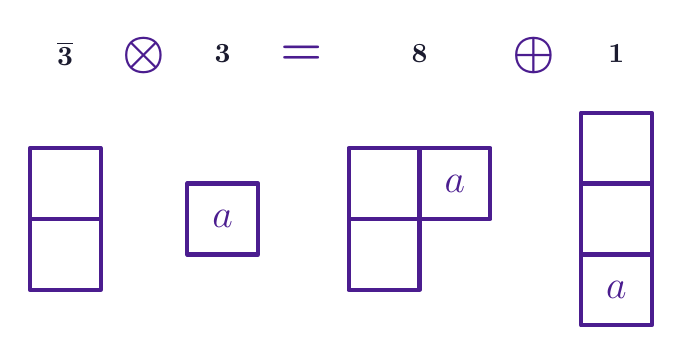
\begin{tikzpicture}[every node/.style={text=ink}]
\node at (0.000,0) {$\overline{\mathbf{3}}$};
\draw[P,line width=1.5pt,line join=round] (-0.450,-1.200) rectangle (0.450,-2.100);
\draw[P,line width=1.5pt,line join=round] (-0.450,-2.100) rectangle (0.450,-3.000);
\node[text=P] at (1.000,-.02) {\LARGE$\bm{\otimes}$};
\node at (2.000,0) {$\mathbf{3}$};
\draw[P,line width=1.5pt,line join=round] (1.550,-1.650) rectangle (2.450,-2.550);
\node[text=P] at (2.000,-2.100) {\Large$a$};
\node[text=P] at (3.000,-.02) {\LARGE$\bm{=}$};
\node at (4.500,0) {$\mathbf{8}$};
\draw[P,line width=1.5pt,line join=round] (3.600,-1.200) rectangle (4.500,-2.100);
\draw[P,line width=1.5pt,line join=round] (4.500,-1.200) rectangle (5.400,-2.100);
\draw[P,line width=1.5pt,line join=round] (3.600,-2.100) rectangle (4.500,-3.000);
\node[text=P] at (4.950,-1.650) {\Large$a$};
\node[text=P] at (5.950,-.02) {\LARGE$\bm{\oplus}$};
\node at (7.000,0) {$\mathbf{1}$};
\draw[P,line width=1.5pt,line join=round] (6.550,-0.750) rectangle (7.450,-1.650);
\draw[P,line width=1.5pt,line join=round] (6.550,-1.650) rectangle (7.450,-2.550);
\draw[P,line width=1.5pt,line join=round] (6.550,-2.550) rectangle (7.450,-3.450);
\node[text=P] at (7.000,-3.000) {\Large$a$};
\end{tikzpicture}
\end{document}
